% Paper source; executable expressions remain in the proof runner.
% Build twice with: xelatex -interaction=nonstopmode -halt-on-error algebraic-retrieval.tex
% arXiv processor: xelatex. Fonts use TeX Live filenames, not fontconfig names.
\documentclass{article}
\usepackage{arxiv}
\usepackage{fontspec}
\setmainfont{texgyretermes-regular.otf}[
  BoldFont=texgyretermes-bold.otf,
  ItalicFont=texgyretermes-italic.otf,
  BoldItalicFont=texgyretermes-bolditalic.otf]
\setsansfont{texgyreheros-regular.otf}[
  BoldFont=texgyreheros-bold.otf,
  ItalicFont=texgyreheros-italic.otf,
  BoldItalicFont=texgyreheros-bolditalic.otf]
\setmonofont{DejaVuSansMono.ttf}[
  BoldFont=DejaVuSansMono-Bold.ttf,
  ItalicFont=DejaVuSansMono-Oblique.ttf,
  BoldItalicFont=DejaVuSansMono-BoldOblique.ttf,
  Scale=0.90]
\usepackage{amsmath,unicode-math}
\setmathfont{texgyretermes-math.otf}
\newcommand{\matmul}{\mathbin{@}}
\usepackage{booktabs,longtable,array}
\usepackage{graphicx}
\usepackage{calc}
\usepackage{xcolor,listings}
\definecolor{CodeBackground}{HTML}{F5F6F8}
\definecolor{CodeRule}{HTML}{B8C4D0}
\definecolor{CodeKeyword}{HTML}{264B70}
\definecolor{CodeString}{HTML}{70513C}
\lstdefinestyle{paper}{
  basicstyle=\ttfamily\fontsize{9}{10.5}\selectfont,
  columns=fullflexible,keepspaces=true,showstringspaces=false,
  upquote=true,breaklines=true,breakatwhitespace=false,
  backgroundcolor=\color{CodeBackground},
  frame=l,rulecolor=\color{CodeRule},framerule=0.6pt,framesep=4pt,
  xleftmargin=6pt,xrightmargin=4pt,
  aboveskip=4pt,belowskip=6pt,
  keywordstyle=\color{CodeKeyword}\bfseries,
  stringstyle=\color{CodeString},commentstyle=\color{gray}\itshape,
  tabsize=4
}
\lstset{style=paper}
\usepackage[font=small,labelfont=bf]{caption}
\setlength{\intextsep}{7pt}
\usepackage{xurl}
\usepackage[hidelinks,unicode]{hyperref}
\hypersetup{pdftitle={Algebraic Retrieval: Composable Search for Agents},pdfauthor={Damian Delmas}}
\providecommand{\tightlist}{\setlength{\itemsep}{0pt}\setlength{\parskip}{0pt}}
\setcounter{secnumdepth}{2}
\renewcommand{\shorttitle}{Algebraic Retrieval}
\title{Algebraic Retrieval: Composable Search for Agents}
\author{Damian Delmas \\
Independent Researcher, Vancouver, BC \\
\texttt{damian@getflex.dev}}
\date{}
\raggedbottom
\setlength{\parskip}{3pt}
\begin{document}
\maketitle
\begin{abstract}
Algebraic Retrieval lets AI agents compose search strategies at query time. Relevance criteria, eligibility constraints, and ranking preferences can be expressed together in a mathematical query. The agent can discover available operations, combine them for the question at hand, and revise its strategy after inspecting the results. This gives the agent control over both what it searches for and how it searches. Building on Programmatic Embedding Modulation (PEM), we demonstrate contrastive scoring, candidate-pool reranking, and weighted ranking as composable queries, alongside executable SQL and PyTerrier counterparts. On the public 11,429-document Vaswani fixture, each program's implementations select the same document set with score differences below \texttt{1e-6}; one tied pair orders differently across scoring paths.
\end{abstract}

\hypertarget{introduction}{%
\section{Introduction}\label{introduction}}

Retrieval is often presented to an agent as one search call with a query and a few parameters. For example, an agent may seek implementation architecture and runtime behavior while suppressing marketing material, restrict candidates to engineering discussions, and weight their scores by recency. These operations can be written together as an expression.

Algebraic Retrieval lets the agent compose that expression at query time. The agent chooses the scoring directions, the eligible records, and how individual scores are weighted. It can revise the program after inspecting its results, using declared symbols instead of reconstructing their underlying joins or Python pipeline bindings. Agreement with established systems checks that the program executes as intended.

The immediate precursor is Programmatic Embedding Modulation (PEM) {[}5{]}, which already combined vector and score operations with SQL pre-filtering in a materializer. Algebraic Retrieval makes their composition explicit in the program the agent writes. The following sections explain the objects involved, what the agent sees through \texttt{orient}, and three retrieval programs expressed in Algebra, SQL, and PyTerrier.

\hypertarget{preliminaries}{%
\section{Preliminaries}\label{preliminaries}}

Let \(E\) contain one embedding per record and \(q\) be a query vector. Then \(E\matmul q\) assigns a similarity score to every candidate. With normalized rows and a unit query, these scores equal cosine similarity. An identity stays attached to each score so that results can be joined to the underlying records.

The arithmetic in this paper uses queries in the same embedding space. \(+\) adds their scores, \(-\) subtracts them, and scalar \texttt{*} scales a contribution. For example, \((E\matmul q_1)-0.5\,(E\matmul q_2)\) favors the first direction while suppressing the second. Selection happens after composition; subtracting two already-truncated top-ten lists would be a different operation. In displayed formulas, \(q_1\) and \(q_2\) denote the source tokens \texttt{q1} and \texttt{q2}.

A mask \(m\) is a set of eligible identities. \(m\triangleright S\) removes other records from a scored relation \(S\). A weight relation \(w\) supplies a scalar for each eligible identity, and \(w\odot S\) multiplies its score. Masks remove records; a zero weight leaves a record present with score zero. Finally, \(\tau_{10}(S)\) selects up to ten results, ordered by score descending and identity ascending. The ASCII spelling is \texttt{top(10,\ S)}.

\hypertarget{architecture}{%
\section{Architecture}\label{architecture}}

The architecture follows PEM's division of work. The current materializer uses SQLite to resolve operands and NumPy to evaluate vector arithmetic, then returns a temporary relation that SQL can hydrate, join, or group. The existing parser and planner determine the operations from the agent's expression.

\begin{figure}[!ht]
\centering
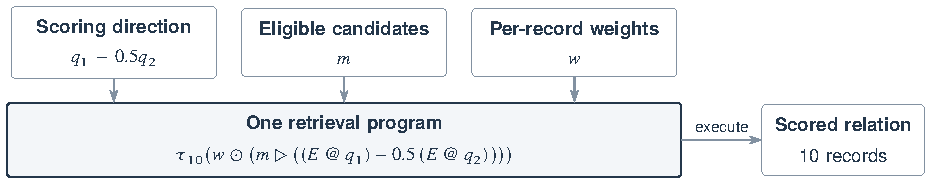
\includegraphics[width=\linewidth]{figures/retrieval-program.pdf}
\caption{An agent combines scoring directions, a candidate mask, and per-record weights into the query of §5.3. Execution returns a scored relation that can be inspected or composed further.}
\label{fig:retrieval-program}
\end{figure}

The agent submits a program through \texttt{algebra(\textquotesingle{}\textless{}expression\textgreater{}\textquotesingle{})}. It can also place that constructor inside a larger SQL query. Changing a subtraction coefficient or adding a mask changes the retrieval program without requiring a new endpoint.

PEM's \texttt{similar:} and \texttt{suppress:} tokens requested numerical operations through SQL. Algebra expresses their composition directly. Before scoring, the planner can collapse:

\[
  (E\matmul q_1)-0.5\,(E\matmul q_2)
  = E\matmul(q_1-0.5q_2).
\]

This identity holds in real arithmetic. The implementation preserves the composed vector's magnitude and performs one matrix multiplication; float32 evaluation orders can differ slightly.

For a fixed \(E\), changing \(q\) leaves the scored identities intact. Masks change that support, while per-record weighting generally cannot be absorbed into a change of \(q\).

The SQL listings below are executable equivalents, not compiler output. They use sqlite-vec {[}10{]} to calculate cosine similarity directly from stored vectors, and run over the fixture's \texttt{embeddings(docno,\ vector)} and the views \texttt{m(id)} and \texttt{w(id,\ weight)} defined at the end of the paper.

\hypertarget{orient-what-the-agent-sees}{%
\section{Orient: what the agent sees}\label{orient-what-the-agent-sees}}

Before writing a query, the agent calls:

\begin{lstlisting}
algebra('orient')
\end{lstlisting}

The response identifies available operands, their underlying relations, and whether they can be used. These are the six operand rows returned for the Vaswani proof fixture:

\begin{longtable}[]{@{}llll@{}}
\toprule\noalign{}
section & token & domain & status \\
\midrule\noalign{}
\endhead
\bottomrule\noalign{}
\endlastfoot
relation & \texttt{R} & \texttt{documents(docno,\ text)} & \texttt{ok} \\
matrix & \texttt{E} & \texttt{embeddings(docno,\ vector)} & \texttt{ok} \\
query & \texttt{q1} & \texttt{query\_vectors(qid,\ vector)} & \texttt{ok} \\
query & \texttt{q2} & \texttt{embeddings(docno,\ vector)} & \texttt{ok} \\
mask & \texttt{m} & \texttt{pyterrier\_bm25\_results(docno,\ qid)} & \texttt{ok} \\
weight & \texttt{w} & \texttt{pyterrier\_bm25\_results(docno,\ score,\ qid)} & \texttt{ok} \\
\end{longtable}

The same response advertises scoring, restriction, weighting, fusion, and selection. The agent sees both usable symbols and their underlying schema. Whoever integrates the corpus declares the bindings between symbols and relations; this fixture declares them in the proof runner. The agent composes within that namespace.

The fixture contains 11,429 documents and deterministic 128-dimensional vectors. \texttt{q1} is the stored query vector for ``What are chemical reactions?''; \texttt{q2} is a fixed vector from document \texttt{2008}. The mask contains the 52 candidates in the recorded PyTerrier BM25 result for that query. Each weight is its BM25 score divided by the maximum score in that result. The vectors make the computation reproducible; they are not a learned-embedding retrieval evaluation.

\newpage

\hypertarget{queries-the-agent-can-compose}{%
\section{Queries the agent can compose}\label{queries-the-agent-can-compose}}

The examples introduce signed scoring and candidate restriction, then combine both with per-record weights. For the PyTerrier forms, \texttt{D} supplies every document, \texttt{M} supplies the recorded BM25 candidates, \texttt{A} and \texttt{B} score with the two query vectors, and \texttt{W} applies the declared weights. \texttt{T} explicitly orders by score and document identity before cutoff. Their native PyTerrier definitions appear at the end of the paper.

\hypertarget{subtract-one-similarity-search-from-another}{%
\subsection{Subtract one similarity search from another}\label{subtract-one-similarity-search-from-another}}

The agent can use a second query or an example document to specify an unwanted direction. Here document \texttt{2008} fixes the subtraction operand reproducibly; it is not assigned an irrelevance judgment.

\textbf{Algebraic expression}

\[
  \tau_{10}\!\left((E\matmul q_1)-0.5\,(E\matmul q_2)\right)
\]

\textbf{Equivalent SQL}

\begin{lstlisting}[language=SQL]
SELECT docno AS id,
       (1 - vec_distance_cosine(vector, :q1))
       - 0.5 * (1 - vec_distance_cosine(vector, :q2)) AS score
FROM embeddings
ORDER BY score DESC, id ASC
LIMIT 10;
\end{lstlisting}

\textbf{PyTerrier}

\begin{lstlisting}[language=Python]
(D >> (A + (-0.5) * B) >> T) % 10
\end{lstlisting}

PyTerrier adds the first scorer to a negatively weighted second scorer. The SQL alternative calculates two primitive cosine similarities per row; Algebra combines the vectors and scores once. All select the same ten identities, with document \texttt{9448} first. PyTerrier returns the same order, with a maximum score difference of \texttt{2.24e-8}. Documents \texttt{7429} and \texttt{9217} tie exactly in Algebra and PyTerrier, where identity ordering places \texttt{7429} first. The SQL path separates them by approximately \texttt{5.96e-8} and places \texttt{9217} first; its maximum returned-score difference is also approximately \texttt{5.96e-8}.

Replacing subtraction with addition expresses a blend. This is the practical meaning of composing searches with \(+\), \(-\), and \texttt{*}: the agent writes the scoring expression it needs.

\hypertarget{rerank-a-candidate-pool}{%
\subsection{Rerank a candidate pool}\label{rerank-a-candidate-pool}}

The agent restricts vector scoring to an existing first-pass result. Here the mask is the 52-document BM25 candidate pool exposed by \texttt{orient}.

\textbf{Algebraic expression}

\[
  \tau_{10}\!\left(m\triangleright(E\matmul q_1)\right)
\]

\textbf{Equivalent SQL}

\begin{lstlisting}[language=SQL]
SELECT e.docno AS id, 1 - vec_distance_cosine(e.vector, :q1) AS score
FROM embeddings AS e JOIN m ON m.id = e.docno
ORDER BY score DESC, id ASC
LIMIT 10;
\end{lstlisting}

\textbf{PyTerrier}

\begin{lstlisting}[language=Python]
(M >> A >> T) % 10
\end{lstlisting}

This is the familiar candidate-generation → reranking → cutoff pipeline. The Algebra planner applies the mask before its vector scoring pass. The SQL join expresses the same allowed identities, and PyTerrier passes those candidates to the scorer. All return the same ordered identities, with document \texttt{2417} first. PyTerrier scores match Algebra exactly; the SQL scores have a maximum observed difference of approximately \texttt{2.98e-8}.

\newpage

\hypertarget{compose-the-full-retrieval-strategy}{%
\subsection{Compose the full retrieval strategy}\label{compose-the-full-retrieval-strategy}}

Within the candidate pool, the agent combines target and suppression scores, applies the declared weights, and selects the top ten. Normalized BM25 weights serve as a mechanical demonstration.

\textbf{Algebraic expression}

\[
  \tau_{10}\!\left(
    w\odot\left(m\triangleright
      \left((E\matmul q_1)-0.5\,(E\matmul q_2)\right)
    \right)
  \right)
\]

\textbf{Equivalent SQL}

\begin{lstlisting}[language=SQL]
SELECT e.docno AS id,
       w.weight * ((1 - vec_distance_cosine(e.vector, :q1))
                   - 0.5 * (1 - vec_distance_cosine(e.vector, :q2))) AS score
FROM embeddings AS e
JOIN m ON m.id = e.docno JOIN w ON w.id = e.docno
ORDER BY score DESC, id ASC
LIMIT 10;
\end{lstlisting}

\textbf{PyTerrier}

\begin{lstlisting}[language=Python]
(M >> (A + (-0.5) * B) >> W >> T) % 10
\end{lstlisting}

All 52 eligible identities have weights. All three forms return the same ordered identities, with document \texttt{10703} first. Maximum score differences relative to Algebra are approximately \texttt{2.98e-8} for SQL and \texttt{1.49e-8} for PyTerrier.

The third program composes the choices introduced earlier: combine scoring directions, restrict the candidates, and apply per-record preferences before selection. Its output remains a scored relation that the agent can inspect and reuse.

\hypertarget{explanation-and-evidence}{%
\section{Explanation and evidence}\label{explanation-and-evidence}}

The composition works because the intermediate scores remain available with their identities. Arithmetic changes their values, a mask changes which identities participate, and top-k selects the final result. The same objects pass between these operations.

The PyTerrier 1.1.2 programs use independent FAISS 1.15.0 \texttt{IndexFlatIP} scores. The SQL alternatives compute scores directly with sqlite-vec 0.1.9 over the stored vectors. Every selected document set matches Algebra and all score differences are below \texttt{1e-6}; §5.1 reports the ordering difference. These are computation checks, not timing comparisons. The candidate pool is the recorded upstream BM25 result, so the checks do not compare BM25 implementations.

Score tolerance does not imply rank agreement. Algebra and PyTerrier tie \texttt{7429} and \texttt{9217} at \texttt{0.24868088960647583}, a reference gap of zero; SQL favors \texttt{9217} by approximately \texttt{5.96e-8}. Identity ordering resolves only computed ties. If each alternative score differs from its reference by at most \(\varepsilon\), a reference gap greater than \(2\varepsilon\) preserves their order.

The uncollapsed §5.2 comparison already shows SQL deviations of approximately \texttt{2.98e-8}. A two-pass NumPy calculation of §5.1 preserves the tie, so this swap does not require collapse. Stored float32 rows are approximately unit length; sqlite-vec 0.1.9 {[}10{]} recomputes norms using float32 accumulation, then rounds cosine distance before SQL subtracts it from one. Reproducing those steps reproduces the pair's split: a deterministic rounding effect.

The existing \href{https://github.com/algebraicretrieval/algebraicretrieval/tree/main/proofs/pyterrier}{six-case proof} also covers score thresholds. Portable regressions check \href{https://github.com/algebraicretrieval/algebraicretrieval/blob/main/tests/test_typed_operators.py}{restriction versus zero-weighting on negative scores} and \href{https://github.com/algebraicretrieval/algebraicretrieval/blob/main/tests/test_score_semantics.py}{identity tie ordering, collapse, and threshold membership}. A \href{https://github.com/algebraicretrieval/algebraicretrieval/blob/main/tests/test_barrier_semantics.py}{feedback regression} executes score → top-1 → centroid → rescore: moving the mask changes the result order, so that stage boundary must be preserved.

PyTerrier already provides an algebra of retrieval transformers {[}3{]}, including \href{https://pyterrier.readthedocs.io/en/latest/transformer.html\#optimisation}{pipeline optimizations}. Here the agent submits one expression over operands discovered through \texttt{orient}; the shared matrix and query terms remain explicit for rewrites such as §3's collapse. Vector scoring and feedback {[}1,2{]}, relational top-k {[}6,7{]}, Vespa ranking expressions {[}8{]}, and semantic relational operators such as LOTUS {[}9{]} supply established context. The experiments do not measure retrieval-quality gains, ANN recall, comparative agent query-writing accuracy, or universal compiler correctness.

\hypertarget{conclusion}{%
\section{Conclusion}\label{conclusion}}

An agent can write retrieval as arithmetic over similarity scores, restrict it with a mask, and change the program at query time. The existing runtime executes these short expressions and returns relations the agent can continue to compose. On the public fixture, three implementations select the same document sets with score differences below \texttt{1e-6}, yet one tied pair orders differently. Numerical agreement must be checked separately from rank agreement.

\newpage

\hypertarget{references}{%
\section*{References}\label{references}}
\addcontentsline{toc}{section}{References}

\begin{enumerate}
\raggedright
\def\labelenumi{\arabic{enumi}.}
\tightlist
\item
  G. Salton, A. Wong, and C. S. Yang. ``A Vector Space Model for Automatic Indexing.'' \emph{Communications of the ACM}, 1975.
\item
  J. J. Rocchio. ``Relevance Feedback in Information Retrieval.'' \emph{The SMART Retrieval System}, 1971.
\item
  Craig Macdonald and Nicola Tonellotto. ``Declarative Experimentation in Information Retrieval using PyTerrier.'' \emph{ICTIR}, 2020.
\item
  Sean MacAvaney et al.~``Simplified Data Wrangling with ir\_datasets.'' \emph{SIGIR}, 2021.
\item
  Damian Delmas. ``flexvec: SQL Vector Retrieval with Programmatic Embedding Modulation.'' arXiv:2603.22587, 2026. DOI: 10.48550/arXiv.2603.22587.
\item
  Chengkai Li, Kevin C.-C. Chang, Ihab F. Ilyas, and Sumin Song. ``RankSQL: Query Algebra and Optimization for Relational Top-k Queries.'' \emph{SIGMOD}, 2005. DOI: 10.1145/1066157.1066173.
\item
  Ronald Fagin, Amnon Lotem, and Moni Naor. ``Optimal Aggregation Algorithms for Middleware.'' \emph{PODS}, 2001. DOI: 10.1145/375551.375567.
\item
  Vespa. ``YQL Query Language,'' ``Ranking Expressions,'' and ``Phased Ranking.'' Vespa Documentation, accessed 2026.
\item
  Liana Patel, Siddharth Jha, Melissa Pan, Harshit Gupta, Parth Asawa, Carlos Guestrin, and Matei Zaharia. ``Semantic Operators and Their Optimization: Enabling LLM-Based Data Processing with Accuracy Guarantees in LOTUS.'' \emph{PVLDB}, 2025.
\item
  Alex Garcia. ``sqlite-vec: API Reference.'' https://alexgarcia.xyz/sqlite-vec/api-reference.html. Version 0.1.9 used in the SQL comparisons; \href{https://github.com/asg017/sqlite-vec/blob/v0.1.9/sqlite-vec.c\#L436}{cosine implementation}.
\end{enumerate}

\hypertarget{example-bindings}{%
\section*{Example bindings}\label{example-bindings}}
\addcontentsline{toc}{section}{Example bindings}

These are the bindings used to check the listings. \texttt{ids} contains all document identities; \texttt{score1} and \texttt{score2} map them to the full independent FAISS primitive scores. \texttt{bm25} contains the recorded first-pass result. Each pipeline is executed with \texttt{.transform(topics)} for the single fixture query.

\begin{lstlisting}[language=Python]
weight = dict(zip(bm25.docno, bm25.score / bm25.score.max()))
D = pt.Transformer.from_df(pd.DataFrame({"qid": "1", "docno": ids}))
M = pt.Transformer.from_df(bm25)
A = pt.apply.doc_score(lambda r: float(score1[r["docno"]]))
B = pt.apply.doc_score(lambda r: float(score2[r["docno"]]))
W = pt.apply.doc_score(lambda r: r["score"] * weight[r["docno"]])

def score_id_order(frame):
    out = frame.sort_values(
        ["score", "docno"], ascending=[False, True], kind="mergesort"
    ).reset_index(drop=True)
    out["rank"] = np.arange(len(out))
    return out

T = pt.apply.generic(score_id_order)
\end{lstlisting}

The explicit ordering stage supplies the comparison's tie policy. PyTerrier's default tied ranks follow input order. Code, fixture instructions {[}4{]}, and dependencies are available at \url{https://github.com/algebraicretrieval/algebraicretrieval/tree/main/proofs/pyterrier}. Its \href{https://github.com/algebraicretrieval/algebraicretrieval/blob/main/proofs/pyterrier/examples.py}{\texttt{examples.py}} runs all three comparisons, the two-pass scoring check, and the scalar rounding reproduction:

\begin{lstlisting}[language=bash]
python proofs/pyterrier/examples.py
\end{lstlisting}

The native SQL alternatives bind \texttt{:q1} to the stored vector for query \texttt{1} and \texttt{:q2} to document \texttt{2008}'s embedding, and use these views. SQL's window maximum and PyTerrier's \texttt{bm25.score.max()} both cover the same 52 rows with \texttt{qid=\textquotesingle{}1\textquotesingle{}}; the maximum is \texttt{22.076426496954774}, and the normalized weights agree exactly.

\begin{lstlisting}[language=SQL]
CREATE TEMP VIEW m AS
SELECT docno AS id FROM pyterrier_bm25_results WHERE qid='1';
CREATE TEMP VIEW w AS
SELECT docno AS id, score / max(score) OVER () AS weight
FROM pyterrier_bm25_results WHERE qid='1';
\end{lstlisting}

\end{document}
